% SOURCE-MATCHED STYLE: adapted from the provided Lecture 4 Beamer format
% Generated: 2026-09-01 +07
% Revised v2: figures checked and refitted to slide/column width
\documentclass[aspectratio=169]{beamer}

\usepackage[utf8]{inputenc}
\usepackage[english]{babel}
\usepackage{amsmath,amssymb}
\usepackage{booktabs}
\usepackage{array}
\usepackage{graphicx}
\usepackage{adjustbox}
\usepackage{listings}
\usepackage{tikz}
\usetikzlibrary{arrows.meta,positioning,shapes.geometric,calc,trees}

\usepackage{empheq}
\usepackage{tcolorbox}
\tcbuselibrary{skins,theorems}

\newtcbox{\mymath}[1][]{%
    nobeforeafter, math upper, tcbox raise base,
    enhanced, colframe=blue!30!black,
    colback=blue!30, boxrule=1pt,
    #1}

\graphicspath{{images/}{figures/}{logo/}{../logo/}}

\definecolor{ForestGreen}{RGB}{22,100,70}
\definecolor{SoftGreen}{RGB}{229,244,235}
\definecolor{SoftBlue}{RGB}{226,239,255}
\definecolor{SoftOrange}{RGB}{255,241,220}
\definecolor{SoftPurple}{RGB}{239,231,255}

\newcolumntype{L}[1]{>{\raggedright\arraybackslash}p{#1}}
\newcolumntype{C}[1]{>{\centering\arraybackslash}p{#1}}

\mode<presentation>{
  \usetheme{Ilmenau}
  \usecolortheme{spruce}
  \usefonttheme{professionalfonts}
  \setbeamertemplate{navigation symbols}{}
  \setbeamertemplate{headline}{}
  \setbeamertemplate{caption}[numbered]
  \setbeamercolor{institute in head/foot}{fg=ForestGreen}
}

\lstset{
  language=Python,
  basicstyle=\ttfamily\footnotesize,
  keywordstyle=\color{blue!75!black}\bfseries,
  stringstyle=\color{red!65!black},
  commentstyle=\color{ForestGreen},
  numbers=left,
  numberstyle=\tiny\color{gray},
  numbersep=6pt,
  showstringspaces=false,
  keepspaces=true,
  columns=fullflexible,
  breaklines=true,
  frame=single,
  rulecolor=\color{ForestGreen!60},
  backgroundcolor=\color{SoftGreen!35},
  tabsize=4
}

\lstdefinestyle{pseudo}{
  basicstyle=\ttfamily\scriptsize,
  keywordstyle=\color{blue!75!black}\bfseries,
  morekeywords={ALGORITHM,FUNCTION,PROCEDURE,INPUT,OUTPUT,IF,THEN,ELSE,
    ELSEIF,RETURN,FOR,EACH,IN,TO,DO,WHILE,REPEAT,UNTIL,END,MOD,DIV,
    CREATE,SET,REMOVE,INFINITY,NONE,TRUE,FALSE,SQRT,LENGTH,CALL},
  numbers=none,
  showstringspaces=false,
  keepspaces=true,
  columns=fullflexible,
  breaklines=true,
  frame=single,
  rulecolor=\color{ForestGreen!60},
  backgroundcolor=\color{SoftBlue!35},
  tabsize=4
}

\lstdefinestyle{pseudonumbered}{
  basicstyle=\ttfamily\scriptsize,
  keywordstyle=\color{blue!75!black}\bfseries,
  morekeywords={ALGORITHM,FUNCTION,PROCEDURE,INPUT,OUTPUT,IF,THEN,ELSE,
    ELSEIF,RETURN,FOR,EACH,IN,TO,DO,WHILE,REPEAT,UNTIL,END,MOD,DIV,
    CREATE,SET,REMOVE,INFINITY,NONE,TRUE,FALSE,SQRT,LENGTH,CALL},
  numbers=left,
  numberstyle=\tiny\color{gray},
  numbersep=6pt,
  showstringspaces=false,
  keepspaces=true,
  columns=fullflexible,
  breaklines=true,
  frame=single,
  rulecolor=\color{ForestGreen!60},
  backgroundcolor=\color{SoftBlue!35},
  tabsize=4
}

\tikzset{
  concept/.style={draw=ForestGreen,rounded corners,fill=SoftGreen,
    very thick,minimum height=1.05cm,text width=3.1cm,align=center},
  process/.style={draw=blue!60!black,rounded corners,fill=SoftBlue,
    thick,minimum height=0.95cm,text width=2.7cm,align=center},
  decision/.style={diamond,draw=orange!75!black,fill=SoftOrange,
    thick,aspect=2.1,text width=2.1cm,align=center,inner sep=1pt},
  data/.style={trapezium,trapezium left angle=70,trapezium right angle=110,
    draw=purple!65!black,fill=SoftPurple,thick,minimum height=0.9cm,
    text width=2.4cm,align=center},
  smallbox/.style={draw=ForestGreen,rounded corners,fill=SoftGreen,
    thick,minimum height=0.85cm,text width=2.2cm,align=center,font=\small},
  tinybox/.style={draw=ForestGreen,rounded corners,fill=SoftGreen,
    thick,minimum height=0.58cm,text width=1.35cm,align=center,font=\tiny},
  orangebox/.style={draw=orange!75!black,rounded corners,fill=SoftOrange,
    thick,minimum height=0.58cm,text width=1.45cm,align=center,font=\tiny},
  bluebox/.style={draw=blue!60!black,rounded corners,fill=SoftBlue,
    thick,minimum height=0.58cm,text width=1.45cm,align=center,font=\tiny},
  arrow/.style={-Latex,very thick,ForestGreen}
}

\newcommand{\TitleLogo}{%
  \IfFileExists{logo/logo_slide.png}{\includegraphics[width=0.27\textwidth]{logo/logo_slide.png}}{%
  \IfFileExists{../logo/logo_slide.png}{\includegraphics[width=0.27\textwidth]{../logo/logo_slide.png}}{%
  \IfFileExists{logo_slide.png}{\includegraphics[width=0.27\textwidth]{logo_slide.png}}{%
  \fcolorbox{ForestGreen}{ForestGreen}{\parbox[c][0.85cm][c]{0.27\textwidth}{\centering\color{white}\bfseries NEU -- DS\&AI}}}}}%
}
\newcommand{\FooterLogo}{%
  \IfFileExists{logo/logo_fda.png}{\includegraphics[width=0.8cm]{logo/logo_fda.png}}{%
  \IfFileExists{../logo/logo_fda.png}{\includegraphics[width=0.8cm]{../logo/logo_fda.png}}{%
  \IfFileExists{logo_fda.png}{\includegraphics[width=0.8cm]{logo_fda.png}}{%
  \fcolorbox{ForestGreen}{ForestGreen}{\parbox[c][0.45cm][c]{0.8cm}{\centering\color{white}\scriptsize FDA}}}}}%
}

\title[DSAI1002 - Part 04]{Data Structures and Algorithms in Python\\Lecture 5: Recursion, Recurrences, and Master Theorem}
\author{Faculty of Data Science and Artificial Intelligence}
\institute{National Economics University}
\date{}

\AtBeginSection[]{
  \begin{frame}[plain]
    \begin{center}
      \vfill
      {\color{ForestGreen}\large\bfseries SECTION \insertsectionnumber}
      \vspace{0.8em}
      {\color{ForestGreen}\rule{0.68\textwidth}{1.2pt}}
      \vspace{1.1em}
      {\usebeamerfont{section title}\color{ForestGreen}\Huge\bfseries
        \insertsectionhead}
      \vspace{1.1em}
      {\color{ForestGreen}\rule{0.68\textwidth}{1.2pt}}
      \vfill
    \end{center}
  \end{frame}
}

\begin{document}

\begin{frame}[plain]
  \setbeamercolor{block body example}{bg=ForestGreen,fg=white}
  \begin{center}
    \begin{beamercolorbox}[wd=\textwidth,sep=1pt,center,rounded=true,shadow=true]{block body example}
      \TitleLogo
    \end{beamercolorbox}
  \end{center}
  \vspace{-0.25em}
  \titlepage
\end{frame}

\logo{\FooterLogo}
\setbeamertemplate{footline}{%
  \begin{beamercolorbox}[colsep=1.5pt]{upper separation line foot}
  \end{beamercolorbox}
  \begin{beamercolorbox}[ht=2.5ex,dp=1.125ex,leftskip=.3cm,rightskip=.3cm]{author in head/foot}%
    \leavevmode{\usebeamerfont{author in head/foot}\insertshortauthor}%
    \hfill%
    {\usebeamerfont{institute in head/foot}\usebeamercolor[fg]{institute in head/foot}\insertshortinstitute}%
    \hfill%
    {\usebeamerfont{institute in head/foot}\usebeamercolor[fg]{institute in head/foot}\insertframenumber{} / \inserttotalframenumber}%
  \end{beamercolorbox}%
  \begin{beamercolorbox}[colsep=1.5pt]{lower separation line foot}
  \end{beamercolorbox}%
}

\begin{frame}{Lecture 5: Table of Contents}
  \tableofcontents[hideallsubsections]
\end{frame}

% =============================================================
\section{Recursive Thinking}
% =============================================================


\begin{frame}{Why Recursion?}
  \begin{columns}[T]
    \begin{column}{0.47\textwidth}
      \begin{alertblock}{Motivation}
        \small
        Many algorithms solve a problem by reducing it to one or more \textbf{smaller problems of the same type}.
        \begin{itemize}\setlength{\itemsep}{0.28em}
          \item search in one half of a sorted array;
          \item sort the left half and right half, then merge;
          \item solve smaller subtrees in a tree;
          \item explore smaller states in dynamic programming.
        \end{itemize}
      \end{alertblock}
    \end{column}
    \begin{column}{0.51\textwidth}
      \begin{center}
        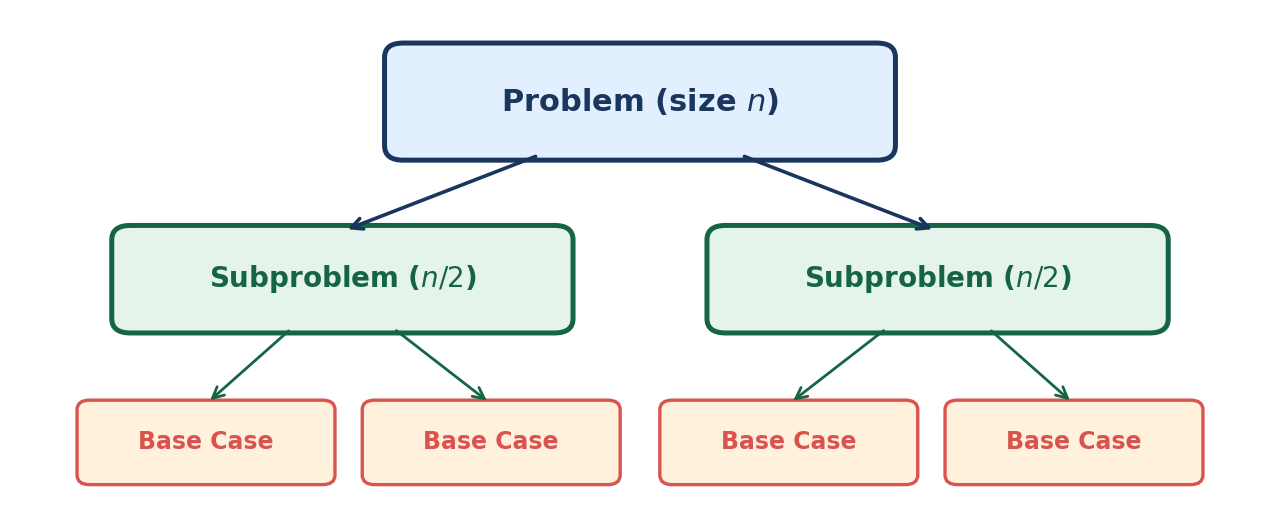
\includegraphics[width=0.98\linewidth]{recursion_figure_assets_v1/page4_clean.png}
      \end{center}
      \vspace{-0.2em}
      \begin{exampleblock}{Key idea}
        \small
        Recursion is natural when the problem has a \textbf{self-similar structure}.
      \end{exampleblock}
    \end{column}
  \end{columns}
\end{frame}


\begin{frame}{Anatomy of a Recursive Algorithm}
  \small
  \begin{columns}[T]
    \begin{column}{0.47\textwidth}
      \begin{block}{Every recursive algorithm needs}
        \begin{enumerate}\setlength{\itemsep}{0.28em}
          \item \textbf{Base case:} solve a small input directly.
          \item \textbf{Recursive case:} reduce to smaller input(s).
          \item \textbf{Progress measure:} strictly decreases.
          \item \textbf{Combination rule:} combine smaller answers.
        \end{enumerate}
      \end{block}
      \begin{alertblock}{Without a base case}
        The function calls itself forever and never returns.
      \end{alertblock}
    \end{column}
    \begin{column}{0.51\textwidth}
      \begin{center}
        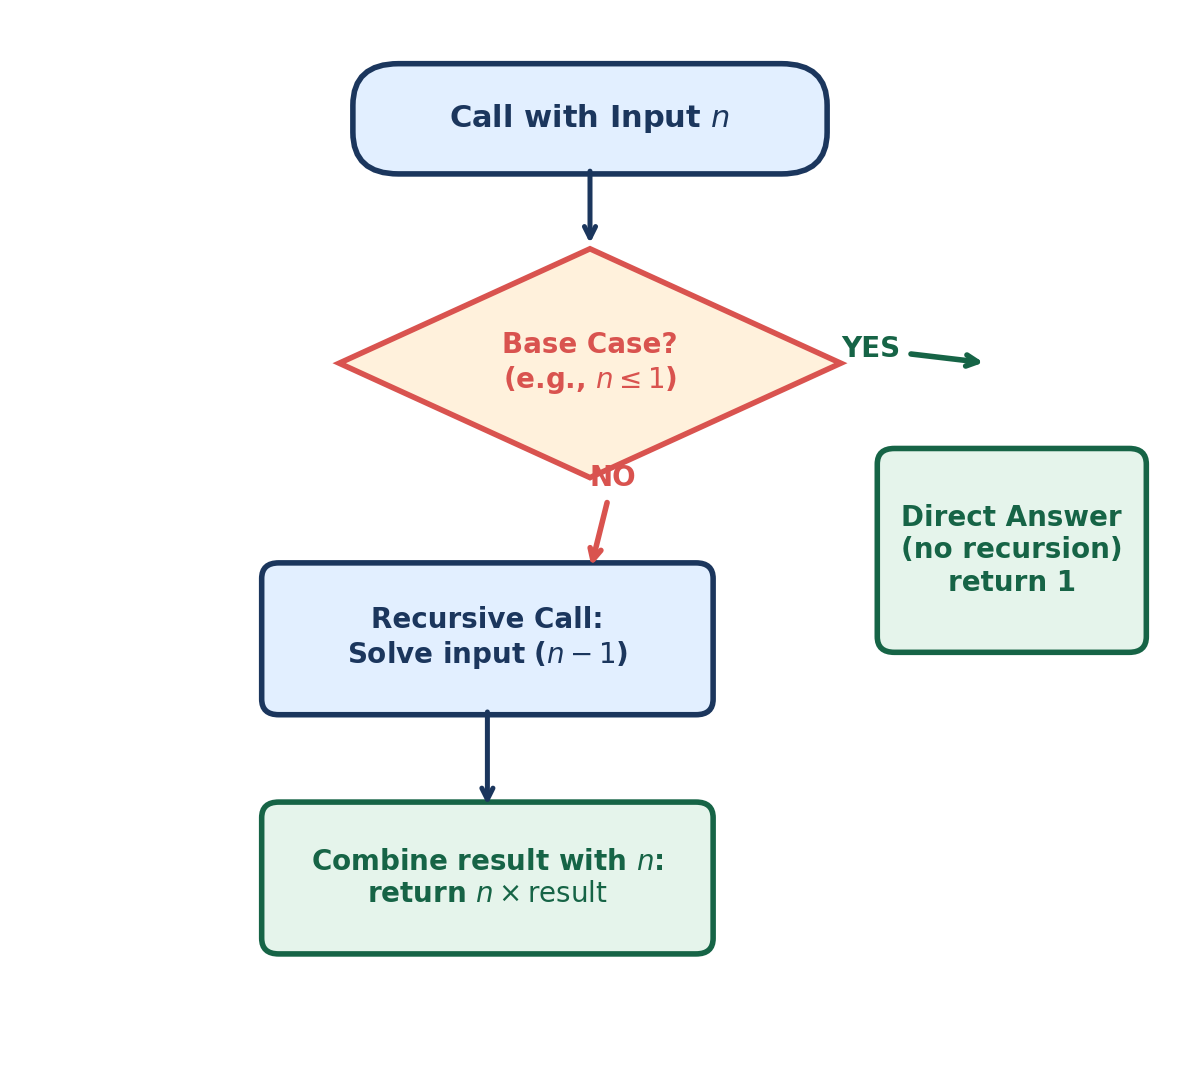
\includegraphics[width=0.99\linewidth]{recursion_figure_assets_v1/page5_clean.png}
      \end{center}
    \end{column}
  \end{columns}
\end{frame}


\begin{frame}[fragile]{Example 1: Factorial}
  \begin{columns}[T]
    \begin{column}{0.53\textwidth}
\begin{lstlisting}[style=pseudonumbered,basicstyle=\ttfamily\scriptsize]
FUNCTION FACTORIAL(n)
INPUT: non-negative integer n
OUTPUT: n!
    IF n == 0 THEN
        RETURN 1
    RETURN n * FACTORIAL(n - 1)
\end{lstlisting}
      \vspace{-0.25em}
      \begin{block}{Mathematical definition}
        \small
        \[
          n! = \begin{cases}
            1, & n=0,\\
            n\cdot(n-1)!, & n>0.
          \end{cases}
        \]
      \end{block}
    \end{column}
    \begin{column}{0.43\textwidth}
      \begin{center}
        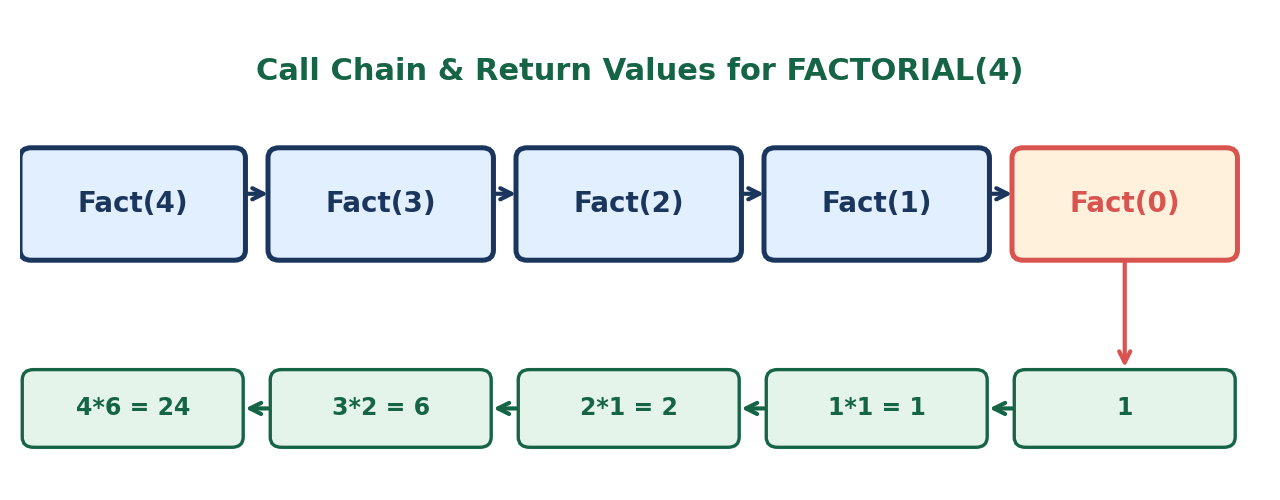
\includegraphics[width=0.84\linewidth]{recursion_figure_assets_v1/page6_clean.png}
      \end{center}
      \vspace{-0.2em}
      \begin{exampleblock}{Running time}
        \small
        One recursive call and constant extra work per level:
        \[
          T(n)=T(n-1)+\Theta(1)=\Theta(n).
        \]
      \end{exampleblock}
    \end{column}
  \end{columns}
\end{frame}

\begin{frame}[fragile]{Example 2: Naive Fibonacci}
  \begin{columns}[T]
    \begin{column}{0.48\textwidth}
\begin{lstlisting}[style=pseudonumbered,basicstyle=\ttfamily\scriptsize]
FUNCTION FIB(n)
INPUT: non-negative integer n
OUTPUT: the n-th Fibonacci number
    IF n <= 1 THEN
        RETURN n
    RETURN FIB(n - 1) + FIB(n - 2)
\end{lstlisting}
      \begin{alertblock}{Why this is expensive}
        \small
        The same subproblems are recomputed many times, such as \texttt{FIB(3)}, \texttt{FIB(2)}, and \texttt{FIB(1)}.
      \end{alertblock}
    \end{column}
    \begin{column}{0.50\textwidth}
      \begin{center}
        \begin{adjustbox}{max width=0.98\linewidth,center}
        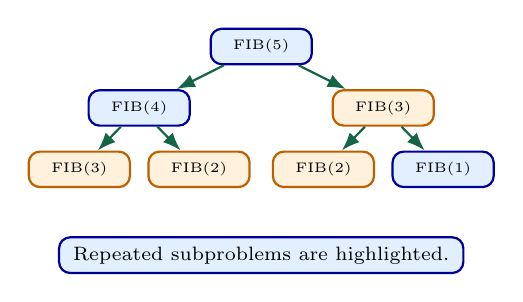
\begin{tikzpicture}[
          level distance=0.78cm,
          level 1/.style={sibling distance=3.10cm},
          level 2/.style={sibling distance=1.52cm},
          every node/.style={bluebox,minimum height=0.45cm,text width=1.05cm,font=\tiny},
          edge from parent/.style={draw,-Latex,thick,ForestGreen}]
          \node {FIB(5)}
            child {node {FIB(4)}
              child {node[orangebox,minimum height=0.45cm,text width=1.05cm,font=\tiny] {FIB(3)}}
              child {node[orangebox,minimum height=0.45cm,text width=1.05cm,font=\tiny] {FIB(2)}}}
            child {node[orangebox,minimum height=0.45cm,text width=1.05cm,font=\tiny] {FIB(3)}
              child {node[orangebox,minimum height=0.45cm,text width=1.05cm,font=\tiny] {FIB(2)}}
              child {node {FIB(1)}}};
          \node[font=\scriptsize,align=center,text width=4.9cm] at (0,-2.65) {Repeated subproblems are highlighted.};
        \end{tikzpicture}
        \end{adjustbox}
      \end{center}
      \begin{exampleblock}{Recurrence}
        \small
        \[
          T(n)=T(n-1)+T(n-2)+\Theta(1),
        \]
        which grows exponentially.
      \end{exampleblock}
    \end{column}
  \end{columns}
\end{frame}

\begin{frame}[fragile]{Example 3: Binary Search}
  \begin{columns}[T]
    \begin{column}{0.55\textwidth}
\begin{lstlisting}[style=pseudonumbered,basicstyle=\ttfamily\scriptsize]
FUNCTION BINARY_SEARCH(A, x, left, right)
INPUT: sorted array A and search value x
OUTPUT: index of x, or NONE
    IF left > right THEN
        RETURN NONE
    mid = (left + right) DIV 2
    IF A[mid] == x THEN
        RETURN mid
    ELSEIF x < A[mid] THEN
        RETURN BINARY_SEARCH(A, x, left, mid - 1)
    ELSE
        RETURN BINARY_SEARCH(A, x, mid + 1, right)
\end{lstlisting}
    \end{column}
    \begin{column}{0.41\textwidth}
      \begin{center}
        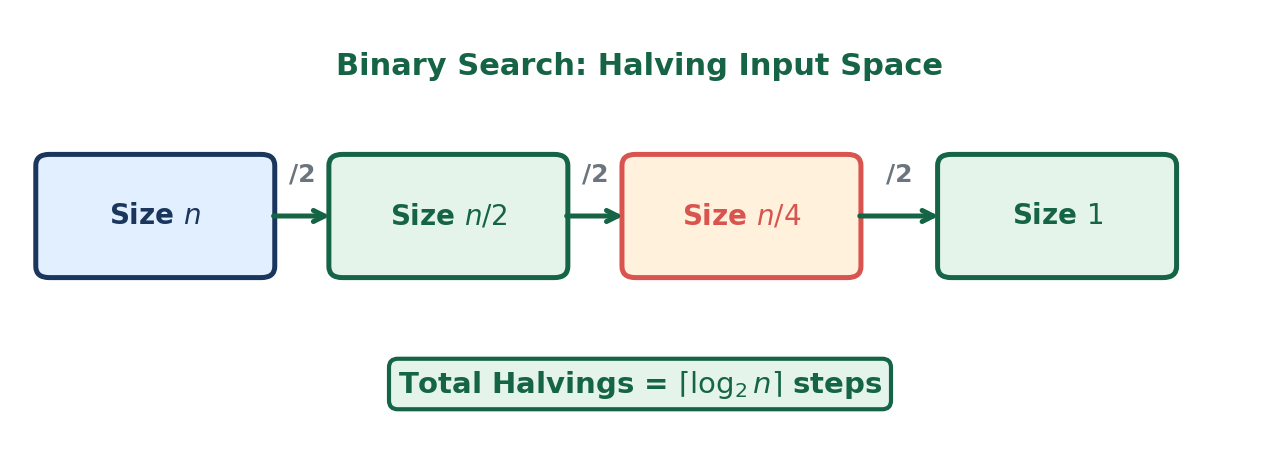
\includegraphics[width=0.97\linewidth]{recursion_figure_assets_v1/page8_clean.png}
      \end{center}
      \begin{exampleblock}{Running time}
        \small
        One recursive call on half the input:
        \[
          T(n)=T(n/2)+\Theta(1)=\Theta(\log n).
        \]
      \end{exampleblock}
    \end{column}
  \end{columns}
\end{frame}

\begin{frame}[fragile]{Example 4: Merge Sort}
  \begin{columns}[T]
    \begin{column}{0.56\textwidth}
\begin{lstlisting}[style=pseudonumbered,basicstyle=\ttfamily\scriptsize]
FUNCTION MERGE_SORT(A)
INPUT: array A of length n
OUTPUT: sorted array containing all elements of A
    IF LENGTH(A) <= 1 THEN
        RETURN A
    mid = LENGTH(A) DIV 2
    left = MERGE_SORT(A[0 .. mid - 1])
    right = MERGE_SORT(A[mid .. n - 1])
    RETURN MERGE(left, right)
\end{lstlisting}
    \end{column}
    \begin{column}{0.40\textwidth}
      \begin{block}{Three-step structure}
        \small
        \begin{enumerate}
          \item \textbf{Divide:} split array into two halves.
          \item \textbf{Conquer:} recursively sort both halves.
          \item \textbf{Combine:} merge two sorted arrays into one sorted result.
        \end{enumerate}
      \end{block}
      \begin{exampleblock}{Recurrence}
        \small
        \[
          T(n)=2T(n/2)+\Theta(n).
        \]
      \end{exampleblock}
    \end{column}
  \end{columns}
\end{frame}

% =============================================================
\section{From Recursion to Recurrence Relations}
% =============================================================

\begin{frame}{What is a Recurrence Relation?}
  \small
  \begin{block}{Definition}
    A \textbf{recurrence relation} expresses the running time for input size $n$ using running times of smaller input sizes.
  \end{block}
  \vspace{0.1em}
  \begin{columns}[T]
    \begin{column}{0.47\textwidth}
      \begin{exampleblock}{Typical forms}
        \[
          T(n)=T(n-1)+\Theta(1)
        \]
        \[
          T(n)=T(n/2)+\Theta(1)
        \]
        \[
          T(n)=2T(n/2)+\Theta(n)
        \]
      \end{exampleblock}
    \end{column}
    \begin{column}{0.49\textwidth}
      \begin{alertblock}{Goal of analysis}
        \small
        The recurrence describes the algorithm structure. We still need to solve it to find a simple growth class such as
        \[
          \Theta(n),\quad \Theta(\log n),\quad \Theta(n\log n),\quad \Theta(2^n).
        \]
      \end{alertblock}
    \end{column}
  \end{columns}
\end{frame}


\begin{frame}{How to Build a Recurrence}
  \small
  \begin{center}
    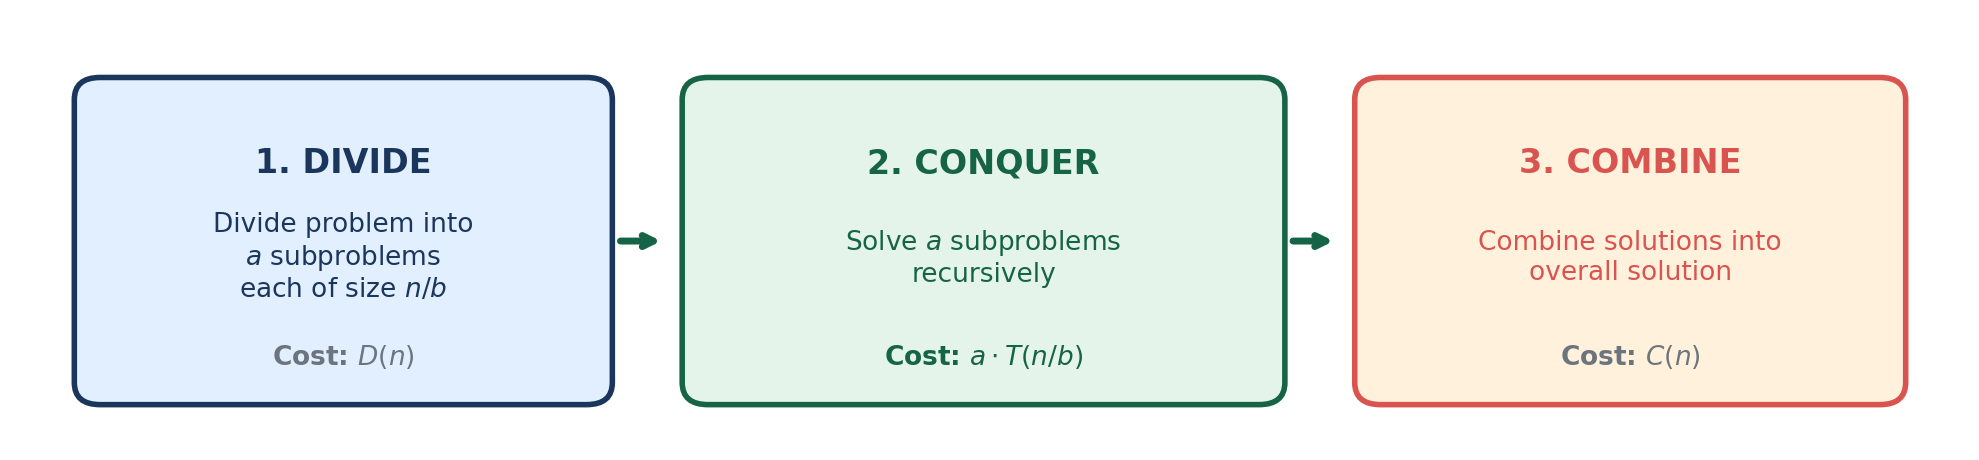
\includegraphics[width=0.96\textwidth]{recursion_figure_assets_v1/page12_clean.png}
  \end{center}
  \vspace{-0.35em}
  \begin{columns}[T]
    \begin{column}{0.49\textwidth}
      \begin{block}{Template for divide-and-conquer}
        \vspace{-0.4em}
        \[
          \mymath{T(n)=aT(n/b)+f(n)}
        \]
        \vspace{-0.7em}
        \begin{itemize}\setlength{\itemsep}{0.08em}
          \item $a$: number of subproblems;
          \item $n/b$: size of each subproblem;
          \item $f(n)$: divide, combine, and other work.
        \end{itemize}
      \end{block}
    \end{column}
    \begin{column}{0.49\textwidth}
      \begin{alertblock}{Do not forget the base case}
        Usually $T(1)=\Theta(1)$ or $T(n)=\Theta(1)$ for $n\le n_0$.
      \end{alertblock}
    \end{column}
  \end{columns}
\end{frame}

\begin{frame}{Examples: Algorithm Structure to Recurrence}
  \small
  \begin{center}
    \renewcommand{\arraystretch}{1.18}
    \begin{tabular}{L{0.28\textwidth}L{0.30\textwidth}L{0.25\textwidth}}
      \toprule
      \textbf{Algorithm} & \textbf{Recursive structure} & \textbf{Recurrence} \\
      \midrule
      Factorial & one call on $n-1$; constant work & $T(n)=T(n-1)+\Theta(1)$ \\
      \addlinespace
      Binary Search & one call on $n/2$; constant work & $T(n)=T(n/2)+\Theta(1)$ \\
      \addlinespace
      Merge Sort & two calls on $n/2$; linear merge & $T(n)=2T(n/2)+\Theta(n)$ \\
      \addlinespace
      Naive Fibonacci & calls on $n-1$ and $n-2$; constant work & $T(n)=T(n-1)+T(n-2)+\Theta(1)$ \\
      \bottomrule
    \end{tabular}
  \end{center}
\end{frame}

\begin{frame}{Recursion Tree: Binary Search}
  \begin{columns}[T]
    \begin{column}{0.54\textwidth}
      \begin{center}
        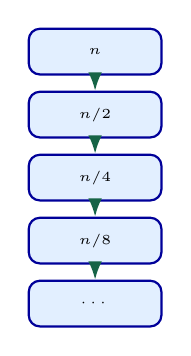
\begin{tikzpicture}[level distance=0.8cm,
          every node/.style={bluebox},
          edge from parent/.style={draw,-Latex,thick,ForestGreen}]
          \node {$n$}
            child {node {$n/2$}
              child {node {$n/4$}
                child {node {$n/8$}
                  child {node {$\cdots$}}}}};
        \end{tikzpicture}
      \end{center}
    \end{column}
    \begin{column}{0.42\textwidth}
      \begin{block}{Cost per level}
        \small
        At each level, there is one subproblem and $\Theta(1)$ non-recursive work.
      \end{block}
      \begin{exampleblock}{Number of levels}
        \small
        Stop when $n/2^k=1$, so $k=\log_2 n$.
        \[
          T(n)=\Theta(\log n).
        \]
      \end{exampleblock}
    \end{column}
  \end{columns}
\end{frame}

\begin{frame}{Recursion Tree: Merge Sort}
  \begin{columns}[T]
    \begin{column}{0.57\textwidth}
      \begin{center}
        \begin{adjustbox}{max width=0.98\linewidth,center}
        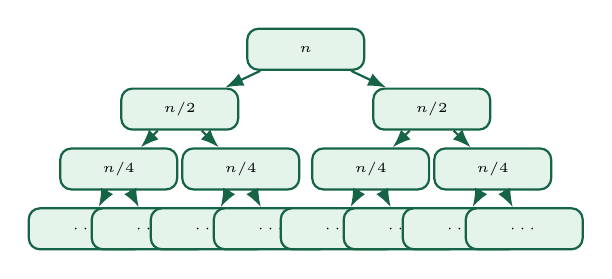
\begin{tikzpicture}[level distance=0.76cm,
          level 1/.style={sibling distance=3.2cm},
          level 2/.style={sibling distance=1.55cm},
          level 3/.style={sibling distance=0.8cm},
          every node/.style={tinybox,minimum height=0.52cm,text width=1.25cm},
          edge from parent/.style={draw,-Latex,thick,ForestGreen}]
          \node {$n$}
            child {node {$n/2$}
              child {node {$n/4$}
                child {node {$\cdots$}}
                child {node {$\cdots$}}}
              child {node {$n/4$}
                child {node {$\cdots$}}
                child {node {$\cdots$}}}}
            child {node {$n/2$}
              child {node {$n/4$}
                child {node {$\cdots$}}
                child {node {$\cdots$}}}
              child {node {$n/4$}
                child {node {$\cdots$}}
                child {node {$\cdots$}}}};
        \end{tikzpicture}
        \end{adjustbox}
      \end{center}
    \end{column}
    \begin{column}{0.40\textwidth}
      \begin{block}{Level cost}
        \centering
        \scriptsize
        \begin{adjustbox}{max width=0.98\linewidth,center}
        \begin{tabular}{c|c|c}
          \toprule
          Level & Subproblems & Total merge cost \\
          \midrule
          $0$ & $1$ of size $n$ & $n$ \\
          $1$ & $2$ of size $n/2$ & $n$ \\
          $2$ & $4$ of size $n/4$ & $n$ \\
          \bottomrule
        \end{tabular}
        \end{adjustbox}
      \end{block}
      \begin{exampleblock}{Conclusion}
        \small
        $\log_2 n$ levels, each costs $\Theta(n)$:
        \[
          T(n)=\Theta(n\log n).
        \]
      \end{exampleblock}
    \end{column}
  \end{columns}
\end{frame}

\begin{frame}{Activity: Build the Recurrence}
  \small
  \begin{block}{Student task}
    For each recursive algorithm pattern, write a recurrence and predict the growth class.
  \end{block}
  \begin{center}
    \renewcommand{\arraystretch}{1.25}
    \begin{tabular}{c|L{0.48\textwidth}|L{0.25\textwidth}}
      \toprule
      & \textbf{Algorithm pattern} & \textbf{Recurrence} \\
      \midrule
      1 & One recursive call on $n-1$ and $\Theta(n)$ work outside & \\
      \addlinespace
      2 & One recursive call on $n/2$ and $\Theta(n)$ work outside & \\
      \addlinespace
      3 & Two recursive calls on $n/2$ and $\Theta(1)$ work outside & \\
      \addlinespace
      4 & Four recursive calls on $n/2$ and $\Theta(n)$ work outside & \\
      \bottomrule
    \end{tabular}
  \end{center}
\end{frame}

% =============================================================
\section{Master Theorem}
% =============================================================

\begin{frame}{Master Theorem: Standard Form}
  \small
  \begin{block}{Recurrence form}
    \[
      \mymath{T(n)=aT(n/b)+f(n)}
    \]
    where $a\ge 1$, $b>1$, and $f(n)$ is non-negative for sufficiently large $n$.
  \end{block}
  \vspace{-0.2em}
  \begin{columns}[T]
    \begin{column}{0.48\textwidth}
      \begin{exampleblock}{The critical comparison}
        \[
          \mymath{n^{\log_b a}}
        \]
        This term represents the growth generated by the recursive branching structure.
      \end{exampleblock}
    \end{column}
    \begin{column}{0.48\textwidth}
      \begin{alertblock}{Intuition}
        Compare \textbf{recursive work} $n^{\log_b a}$ against \textbf{extra work} $f(n)$.
        The larger component usually determines the final complexity.
      \end{alertblock}
    \end{column}
  \end{columns}
\end{frame}

\begin{frame}{Master Theorem: Three Cases}
  \scriptsize
  \begin{center}
    \renewcommand{\arraystretch}{1.23}
    \begin{tabular}{C{0.13\textwidth}L{0.43\textwidth}L{0.26\textwidth}}
      \toprule
      \textbf{Case} & \textbf{Condition} & \textbf{Result} \\
      \midrule
      1 & If $f(n)=O\!\left(n^{\log_b a-\varepsilon}\right)$ for some $\varepsilon>0$ & $T(n)=\Theta\!\left(n^{\log_b a}\right)$ \\
      \addlinespace
      2 & If $f(n)=\Theta\!\left(n^{\log_b a}\log^k n\right)$ for $k\ge 0$ & $T(n)=\Theta\!\left(n^{\log_b a}\log^{k+1} n\right)$ \\
      \addlinespace
      3 & If $f(n)=\Omega\!\left(n^{\log_b a+\varepsilon}\right)$ and $a f(n/b)\le c f(n)$ for some $c<1$ & $T(n)=\Theta(f(n))$ \\
      \bottomrule
    \end{tabular}
  \end{center}
  \vspace{0.25em}
  \begin{alertblock}{Memory aid}
    \centering\small
    Recursive work dominates $\Rightarrow$ balanced $\Rightarrow$ non-recursive work dominates.
  \end{alertblock}
\end{frame}


\begin{frame}{Visual Intuition for the Three Cases}
  \scriptsize
  \begin{columns}[T,onlytextwidth]
    \begin{column}{0.32\textwidth}
      \begin{tcolorbox}[colframe=blue!70!black,colback=SoftBlue!20,title={\centering\bfseries Case 1: leaves},arc=2mm]
        \centering
        \begin{adjustbox}{max width=0.95\linewidth,center}
        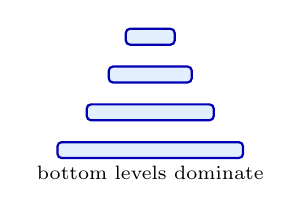
\begin{tikzpicture}[x=0.62cm,y=0.48cm]
          \foreach \y/\w in {3/1.0,2/1.7,1/2.6,0/3.8}{
            \draw[fill=SoftBlue,draw=blue!70!black,thick,rounded corners=1.5pt]
              (2-\w/2,\y) rectangle (2+\w/2,\y+0.42);}
          \node[font=\scriptsize] at (2,-0.40) {bottom levels dominate};
        \end{tikzpicture}
        \end{adjustbox}
        \[
          T(n)=\Theta(n^{\log_b a})
        \]
      \end{tcolorbox}
    \end{column}
    \begin{column}{0.32\textwidth}
      \begin{tcolorbox}[colframe=ForestGreen,colback=SoftGreen!25,title={\centering\bfseries Case 2: balanced},arc=2mm]
        \centering
        \begin{adjustbox}{max width=0.95\linewidth,center}
        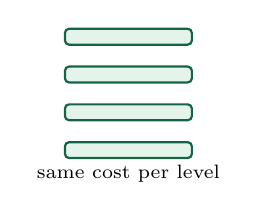
\begin{tikzpicture}[x=0.62cm,y=0.48cm]
          \foreach \y in {3,2,1,0}{
            \draw[fill=SoftGreen,draw=ForestGreen,thick,rounded corners=1.5pt]
              (0.70,\y) rectangle (3.30,\y+0.42);}
          \node[font=\scriptsize] at (2,-0.40) {same cost per level};
        \end{tikzpicture}
        \end{adjustbox}
        \[
          T(n)=\Theta(n^{\log_b a}\log n)
        \]
      \end{tcolorbox}
    \end{column}
    \begin{column}{0.32\textwidth}
      \begin{tcolorbox}[colframe=orange!85!black,colback=SoftOrange!25,title={\centering\bfseries Case 3: root},arc=2mm]
        \centering
        \begin{adjustbox}{max width=0.95\linewidth,center}
        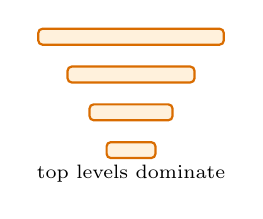
\begin{tikzpicture}[x=0.62cm,y=0.48cm]
          \foreach \y/\w in {3/3.8,2/2.6,1/1.7,0/1.0}{
            \draw[fill=SoftOrange,draw=orange!85!black,thick,rounded corners=1.5pt]
              (2-\w/2,\y) rectangle (2+\w/2,\y+0.42);}
          \node[font=\scriptsize] at (2,-0.40) {top levels dominate};
        \end{tikzpicture}
        \end{adjustbox}
        \[
          T(n)=\Theta(f(n))
        \]
      \end{tcolorbox}
    \end{column}
  \end{columns}
\end{frame}

\begin{frame}{Procedure for Applying Master Theorem}
  \begin{columns}[T]
    \begin{column}{0.48\textwidth}
      \begin{block}{Four steps}
        \small
        \begin{enumerate}
          \item Identify $a$, $b$, and $f(n)$.
          \item Compute $n^{\log_b a}$.
          \item Compare $f(n)$ with $n^{\log_b a}$.
          \item Select the matching case and conclude $T(n)$.
        \end{enumerate}
      \end{block}
      \begin{alertblock}{Important}
        \small
        Do not look only at the number of subproblems. The combine cost $f(n)$ can change the answer.
      \end{alertblock}
    \end{column}
    \begin{column}{0.50\textwidth}
      \begin{center}
        \begin{adjustbox}{max width=0.78\linewidth,center}
        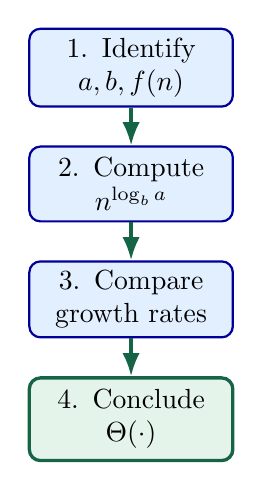
\begin{tikzpicture}[node distance=0.48cm]
          \node[process,text width=2.35cm] (s1) {1. Identify\\$a,b,f(n)$};
          \node[process,text width=2.35cm,below=of s1] (s2) {2. Compute\\$n^{\log_b a}$};
          \node[process,text width=2.35cm,below=of s2] (s3) {3. Compare\\growth rates};
          \node[concept,text width=2.35cm,below=of s3] (s4) {4. Conclude\\$\Theta(\cdot)$};
          \draw[arrow] (s1) -- (s2);
          \draw[arrow] (s2) -- (s3);
          \draw[arrow] (s3) -- (s4);
        \end{tikzpicture}
        \end{adjustbox}
      \end{center}
    \end{column}
  \end{columns}
\end{frame}

\begin{frame}{Example: Merge Sort via Master Theorem}
  \small
  \begin{block}{Recurrence}
    \[
      T(n)=2T(n/2)+\Theta(n)
    \]
  \end{block}
  \begin{columns}[T]
    \begin{column}{0.48\textwidth}
      \begin{exampleblock}{Step-by-step}
        \begin{itemize}
          \item $a=2$, $b=2$, $f(n)=\Theta(n)$.
          \item $n^{\log_b a}=n^{\log_2 2}=n$.
          \item $f(n)=\Theta(n)$ matches the critical term.
          \item Balanced case with $k=0$.
        \end{itemize}
      \end{exampleblock}
    \end{column}
    \begin{column}{0.48\textwidth}
      \begin{alertblock}{Conclusion}
        \[
          T(n)=\Theta(n\log n).
        \]
      \end{alertblock}
      \begin{tcolorbox}[colframe=ForestGreen,colback=SoftGreen!35,arc=1.5mm]
        \centering\small
        The extra $\log n$ factor appears because there are $\log n$ levels, each with total cost $\Theta(n)$.
      \end{tcolorbox}
    \end{column}
  \end{columns}
\end{frame}

\begin{frame}{Example: Recursive Work Dominates}
  \small
  \begin{block}{Recurrence}
    \[
      T(n)=8T(n/2)+n^2
    \]
  \end{block}
  \begin{columns}[T]
    \begin{column}{0.50\textwidth}
      \begin{exampleblock}{Analysis}
        \begin{itemize}
          \item $a=8$, $b=2$, $f(n)=n^2$.
          \item $n^{\log_2 8}=n^3$.
          \item $n^2=O(n^{3-\varepsilon})$ with $\varepsilon=1$.
        \end{itemize}
      \end{exampleblock}
    \end{column}
    \begin{column}{0.46\textwidth}
      \begin{alertblock}{Case 1}
        \centering
        Recursive branching is stronger than the work outside recursive calls.
        \[
          T(n)=\Theta(n^3).
        \]
      \end{alertblock}
    \end{column}
  \end{columns}
\end{frame}

\begin{frame}{Example: Non-recursive Work Dominates}
  \small
  \begin{block}{Recurrence}
    \[
      T(n)=2T(n/2)+n^2
    \]
  \end{block}
  \begin{columns}[T]
    \begin{column}{0.50\textwidth}
      \begin{exampleblock}{Analysis}
        \begin{itemize}
          \item $a=2$, $b=2$, $f(n)=n^2$.
          \item $n^{\log_2 2}=n$.
          \item $n^2=\Omega(n^{1+\varepsilon})$ with $\varepsilon=1$.
          \item Regularity: $2(n/2)^2=n^2/2\le c n^2$ for $c=1/2$.
        \end{itemize}
      \end{exampleblock}
    \end{column}
    \begin{column}{0.46\textwidth}
      \begin{alertblock}{Case 3}
        \centering
        Extra work outside recursion dominates.
        \[
          T(n)=\Theta(n^2).
        \]
      \end{alertblock}
    \end{column}
  \end{columns}
\end{frame}

\begin{frame}{Quick Check: Which Case?}
  \small
  \begin{block}{Exercise}
    For each recurrence, identify $a$, $b$, $f(n)$, the Master Theorem case, and the final bound.
  \end{block}
  \begin{center}
    \renewcommand{\arraystretch}{1.22}
    \begin{tabular}{c|L{0.43\textwidth}|C{0.16\textwidth}|C{0.16\textwidth}}
      \toprule
      & \textbf{Recurrence} & \textbf{Case} & \textbf{Result} \\
      \midrule
      1 & $T(n)=3T(n/2)+n^2$ & & \\
      \addlinespace
      2 & $T(n)=4T(n/2)+n^2$ & & \\
      \addlinespace
      3 & $T(n)=16T(n/4)+n$ & & \\
      \addlinespace
      4 & $T(n)=3T(n/2)+n$ & & \\
      \bottomrule
    \end{tabular}
  \end{center}
\end{frame}

% =============================================================
\section{Extended Master Theorem}
% =============================================================

\begin{frame}{Extended Form: $f(n)=\Theta(n^k\log^p n)$}
  \small
  \begin{block}{Common exercise form}
    \[
      T(n)=aT(n/b)+\Theta(n^k\log^p n).
    \]
  \end{block}
  \vspace{-0.1em}
  \begin{columns}[T]
    \begin{column}{0.48\textwidth}
      \begin{exampleblock}{Shortcut comparison}
        Instead of comparing $f(n)$ with $n^{\log_b a}$ directly, compare
        \[
          a \quad \text{with} \quad b^k.
        \]
      \end{exampleblock}
    \end{column}
    \begin{column}{0.48\textwidth}
      \begin{alertblock}{Why it works}
        \small
        The critical exponent is $\log_b a$. Comparing $a$ and $b^k$ is equivalent to comparing $\log_b a$ and $k$.
      \end{alertblock}
    \end{column}
  \end{columns}
\end{frame}

\begin{frame}{Extended Master Theorem: Summary Table}
  \scriptsize
  \begin{center}
    \renewcommand{\arraystretch}{1.25}
    \begin{tabular}{L{0.31\textwidth}L{0.46\textwidth}}
      \toprule
      \textbf{Condition} & \textbf{Result} \\
      \midrule
      $a>b^k$ & $T(n)=\Theta\!\left(n^{\log_b a}\right)$ \\
      \addlinespace
      $a=b^k$, $p>-1$ & $T(n)=\Theta\!\left(n^k\log^{p+1}n\right)$ \\
      \addlinespace
      $a=b^k$, $p=-1$ & $T(n)=\Theta\!\left(n^k\log\log n\right)$ \\
      \addlinespace
      $a=b^k$, $p<-1$ & $T(n)=\Theta(n^k)$ \\
      \addlinespace
      $a<b^k$, $p\ge 0$ & $T(n)=\Theta\!\left(n^k\log^p n\right)$ \\
      \addlinespace
      $a<b^k$, $p<0$ & typically $O(n^k)$; tight bound requires additional verification \\
      \bottomrule
    \end{tabular}
  \end{center}
  \begin{alertblock}{Teaching note}
    \centering\small
    The boundary $p=-1$ produces the special term $\log\log n$.
  \end{alertblock}
\end{frame}

\begin{frame}{Example: $T(n)=2T(n/2)+n\log n$}
  \small
  \begin{columns}[T]
    \begin{column}{0.50\textwidth}
      \begin{block}{Identify parameters}
        \[
          a=2,\quad b=2,\quad f(n)=n\log n.
        \]
        Here $f(n)=\Theta(n^k\log^p n)$ with
        \[
          k=1,\quad p=1.
        \]
      \end{block}
    \end{column}
    \begin{column}{0.46\textwidth}
      \begin{exampleblock}{Compare}
        \[
          a=2,\qquad b^k=2^1=2.
        \]
        Balanced case: $a=b^k$ and $p>-1$.
      \end{exampleblock}
      \begin{alertblock}{Conclusion}
        \[
          T(n)=\Theta(n\log^{2}n).
        \]
      \end{alertblock}
    \end{column}
  \end{columns}
\end{frame}

\begin{frame}{Example: Boundary Case $p=-1$}
  \small
  \begin{block}{Recurrence}
    \[
      T(n)=2T(n/2)+\frac{n}{\log n}.
    \]
  \end{block}
  \begin{columns}[T]
    \begin{column}{0.49\textwidth}
      \begin{exampleblock}{Parameters}
        \[
          a=2,
          \quad b=2,
          \quad k=1,
          \quad p=-1.
        \]
        Since $a=b^k$, this is a balanced boundary case.
      \end{exampleblock}
    \end{column}
    \begin{column}{0.47\textwidth}
      \begin{alertblock}{Conclusion}
        \[
          T(n)=\Theta(n\log\log n).
        \]
      \end{alertblock}
      \begin{tcolorbox}[colframe=orange!85!black,colback=SoftOrange!35,arc=1.5mm]
        \small
        This result is slower than $\Theta(n)$ but faster than $\Theta(n\log n)$.
      \end{tcolorbox}
    \end{column}
  \end{columns}
\end{frame}

\begin{frame}{Representative Examples}
  \scriptsize
  \begin{center}
    \renewcommand{\arraystretch}{1.18}
    \begin{tabular}{c|L{0.40\textwidth}|L{0.22\textwidth}|L{0.18\textwidth}}
      \toprule
      & \textbf{Recurrence} & \textbf{Result} & \textbf{Remark} \\
      \midrule
      1 & $T(n)=3T(n/2)+n^2$ & $\Theta(n^2)$ & outside work dominates \\
      2 & $T(n)=4T(n/2)+n^2$ & $\Theta(n^2\log n)$ & balanced \\
      3 & $T(n)=4T(n/2)+\log n$ & $\Theta(n^2)$ & recursion dominates \\
      4 & $T(n)=2T(n/2)+n\log n$ & $\Theta(n\log^2 n)$ & $p=1$ \\
      5 & $T(n)=2T(n/2)+n/\log n$ & $\Theta(n\log\log n)$ & $p=-1$ \\
      6 & $T(n)=3T(n/2)+n$ & $\Theta(n^{\log_2 3})$ & recursion dominates \\
      \bottomrule
    \end{tabular}
  \end{center}
\end{frame}

\begin{frame}{Quick Check: Extended Form}
  \small
  \begin{block}{Exercise}
    Solve each recurrence using the extended form when possible.
  \end{block}
  \begin{center}
    \renewcommand{\arraystretch}{1.23}
    \begin{tabular}{c|L{0.46\textwidth}|C{0.16\textwidth}|C{0.17\textwidth}}
      \toprule
      & \textbf{Recurrence} & \textbf{Compare} & \textbf{Result} \\
      \midrule
      1 & $T(n)=2T(n/2)+n\log^2 n$ & & \\
      \addlinespace
      2 & $T(n)=2T(n/2)+n/\log^2 n$ & & \\
      \addlinespace
      3 & $T(n)=6T(n/3)+n^2\log n$ & & \\
      \addlinespace
      4 & $T(n)=3T(n/4)+n\log n$ & & \\
      \bottomrule
    \end{tabular}
  \end{center}
\end{frame}

% =============================================================
\section{Beyond the Standard Master Theorem}
% =============================================================

\begin{frame}{When Master Theorem Cannot Be Applied Directly}
  \small
  \begin{columns}[T]
    \begin{column}{0.48\textwidth}
      \begin{alertblock}{Not in standard form}
        \begin{itemize}
          \item non-constant number of subproblems: $2^nT(n/2)+n^n$;
          \item non-uniform subproblem sizes: $T(n/3)+T(2n/3)+n$;
          \item subtract-and-conquer: $T(n)=T(n-1)+n$;
          \item negative $f(n)$ or failed regularity condition;
          \item coefficient $a<1$ in the standard theorem.
        \end{itemize}
      \end{alertblock}
    \end{column}
    \begin{column}{0.48\textwidth}
      \begin{exampleblock}{Alternative tools}
        \begin{itemize}
          \item recursion tree;
          \item substitution and induction;
          \item direct summation;
          \item variable transformation;
          \item Akra--Bazzi theorem for unequal splits.
        \end{itemize}
      \end{exampleblock}
    \end{column}
  \end{columns}
\end{frame}

\begin{frame}{Subtract-and-Conquer Recurrences}
  \small
  \begin{block}{Typical form}
    \[
      T(n)=aT(n-b)+f(n).
    \]
    The input size decreases by a fixed amount, not by a constant fraction.
  \end{block}
  \begin{center}
    \renewcommand{\arraystretch}{1.2}
    \begin{tabular}{L{0.30\textwidth}L{0.38\textwidth}}
      \toprule
      \textbf{Recurrence} & \textbf{Result} \\
      \midrule
      $T(n)=T(n-1)+1$ & $\Theta(n)$ \\
      \addlinespace
      $T(n)=T(n-1)+n$ & $\Theta(n^2)$ \\
      \addlinespace
      $T(n)=2T(n-1)+1$ & $\Theta(2^n)$ \\
      \bottomrule
    \end{tabular}
  \end{center}
  \begin{alertblock}{Main idea}
    \centering\small
    Expand the recurrence until reaching the base case, then sum the work across levels.
  \end{alertblock}
\end{frame}

\begin{frame}{Example: $T(n)=T(n-1)+n$}
  \small
  \begin{columns}[T]
    \begin{column}{0.52\textwidth}
      \begin{block}{Expansion}
        \[
        \begin{aligned}
          T(n)&=T(n-1)+n\\
              &=T(n-2)+(n-1)+n\\
              &=T(n-3)+(n-2)+(n-1)+n\\
              &\cdots\\
              &=T(1)+2+3+\cdots+n.
        \end{aligned}
        \]
      \end{block}
    \end{column}
    \begin{column}{0.44\textwidth}
      \begin{exampleblock}{Summation}
        \[
          1+2+\cdots+n=\frac{n(n+1)}{2}=\Theta(n^2).
        \]
      \end{exampleblock}
      \begin{alertblock}{Conclusion}
        \[
          T(n)=\Theta(n^2).
        \]
      \end{alertblock}
    \end{column}
  \end{columns}
\end{frame}

\begin{frame}{Guess-and-Prove Method}
  \small
  \begin{block}{Method}
    When no direct theorem applies, guess the solution form and prove it by mathematical induction.
  \end{block}
  \begin{columns}[T]
    \begin{column}{0.48\textwidth}
      \begin{enumerate}
        \item Observe the recurrence and guess a growth class.
        \item Assume the hypothesis holds for smaller inputs.
        \item Substitute the hypothesis into the recurrence.
        \item Verify the inequality for sufficiently large $n$.
      \end{enumerate}
    \end{column}
    \begin{column}{0.48\textwidth}
      \begin{alertblock}{If the proof fails}
        \small
        The guess may need stronger constants, a correction term, or a different growth class.
      \end{alertblock}
      \begin{exampleblock}{Common use}
        \small
        Proving upper bounds such as $T(n)\le cn\log n$ or lower bounds such as $T(n)\ge cn$.
      \end{exampleblock}
    \end{column}
  \end{columns}
\end{frame}

\begin{frame}{Example Beyond Master Theorem}
  \small
  \begin{block}{Recurrence}
    \[
      T(n)=\sqrt{n}\,T(\sqrt{n})+n.
    \]
    Standard Master Theorem does not apply because the number of subproblems $\sqrt n$ is not constant.
  \end{block}
  \begin{columns}[T]
    \begin{column}{0.48\textwidth}
      \begin{exampleblock}{Transformation}
        Let $U(n)=T(n)/n$. Then
        \[
          U(n)=U(\sqrt n)+1.
        \]
        Arguments shrink as
        \[
          n,\sqrt n,n^{1/4},n^{1/8},\ldots
        \]
      \end{exampleblock}
    \end{column}
    \begin{column}{0.48\textwidth}
      \begin{alertblock}{Number of levels}
        Stop when $n^{1/2^k}$ is constant, so $2^k=\Theta(\log n)$ and
        \[
          k=\Theta(\log\log n).
        \]
        Hence
        \[
          T(n)=\Theta(n\log\log n).
        \]
      \end{alertblock}
    \end{column}
  \end{columns}
\end{frame}

% =============================================================
\section{Practice and Key Takeaways}
% =============================================================

\begin{frame}{Practice Exercises}
  \small
  \begin{block}{Solve the following recurrences}
    \begin{enumerate}
      \item $T(n)=8T(n/2)+n^2$.
      \item $T(n)=2T(n/2)+n\log^2 n$.
      \item $T(n)=2T(n/2)+n/\log n$.
      \item $T(n)=4T(n/2)+\log n$.
      \item $T(n)=T(n-1)+n$.
      \item $T(n)=\sqrt n\,T(\sqrt n)+n$.
      \item Explain why $T(n)=T(n/3)+T(2n/3)+n$ does not fit the standard Master Theorem.
    \end{enumerate}
  \end{block}
\end{frame}

\begin{frame}{Self-Test Quiz}
  \scriptsize
  \begin{center}
    \renewcommand{\arraystretch}{1.18}
    \begin{tabular}{c|L{0.56\textwidth}|L{0.20\textwidth}}
      \toprule
      & \textbf{Question} & \textbf{Answer} \\
      \midrule
      1 & $T(n)=4T(n/2)+n^2$ & \\
      \addlinespace
      2 & $T(n)=2T(n/2)+n/\log n$ & \\
      \addlinespace
      3 & Which one does not fit standard Master Theorem: $2T(n/2)+n$, $4T(n/2)+n^2$, $T(n/3)+T(2n/3)+n$? & \\
      \addlinespace
      4 & $T(n)=T(n-1)+n$ & \\
      \addlinespace
      5 & $T(n)=\sqrt n\,T(\sqrt n)+n$ & \\
      \bottomrule
    \end{tabular}
  \end{center}
\end{frame}

\begin{frame}{Common Mistakes}
  \small
  \begin{columns}[T]
    \begin{column}{0.48\textwidth}
      \begin{alertblock}{Mistake 1: Ignore $f(n)$}
        \small
        $T(n)=2T(n/2)+n$ and $T(n)=2T(n/2)+n^2$ have the same recursive calls but different final complexities.
      \end{alertblock}
      \begin{alertblock}{Mistake 2: Apply Master Theorem to any recurrence}
        \small
        Unequal splits, subtract-and-conquer, or non-constant $a$ require other methods.
      \end{alertblock}
    \end{column}
    \begin{column}{0.48\textwidth}
      \begin{alertblock}{Mistake 3: Forget base cases}
        \small
        Recursive algorithms must terminate; recurrence relations usually assume $T(1)=\Theta(1)$.
      \end{alertblock}
      \begin{alertblock}{Mistake 4: Confuse $O$ and $\Theta$}
        \small
        Master Theorem usually gives a tight $\Theta$ bound, not only an upper bound.
      \end{alertblock}
    \end{column}
  \end{columns}
\end{frame}

\begin{frame}{Key Takeaways}
  \small
  \begin{itemize}
    \setlength{\itemsep}{0.35em}
    \item \textbf{Recursion} solves a problem by calling the same procedure on smaller inputs.
    \item Every recursive algorithm needs a \textbf{base case}, a \textbf{recursive case}, and a decreasing progress measure.
    \item A \textbf{recurrence relation} describes how running time depends on smaller input sizes.
    \item For divide-and-conquer recurrences $T(n)=aT(n/b)+f(n)$, compare $f(n)$ with $n^{\log_b a}$.
    \item Master Theorem has three main outcomes: recursive work dominates, balanced work, or non-recursive work dominates.
    \item The extended form $f(n)=\Theta(n^k\log^p n)$ handles many logarithmic variations.
    \item Not all recurrences fit the standard theorem; use recursion trees, summations, transformations, or induction when needed.
  \end{itemize}
\end{frame}

\end{document}
